``rmt'' or Ross's Monitoring Tool is a network monitoring tool 
designed to work with the University of Glasgow's Raspberry Pi 
Cloud. It's primary purpose is to provide an at-a-glance view of the 
status and resource usage of each Raspberry Pi and their respective 
Linux containers.

\section{University of Glasgow Raspberry Pi Cloud}
\label{intro:picloud}

The University of Glasgow's Raspberry Pi Cloud \citep{glapicloud, picloudblog} (which will now be 
referred to as PiCloud, not to be confused with PiCloud Inc. \citeyearpar{picloudinc}) is an effort by the University of Glasgow to replicate Warehouse Scale Computing (WSC) [reference] on a number of Raspberry Pi \citep{rasppi} devices to create a small-scale cloud [cloud reference?].
This was implemented using a software stack consisting of various tools such as LXC \citeyearpar{lxc}running on the Pi devices, each communicating to a ``Pi Master'' which is a regular PC server.
Prior to the creation of \emph{rmt} no monitoring tool was in use, meaning that no user feedback was received when, for example, a host stopped communicating to the Pi Master.
Currently the PiCloud consists of 56 Raspberry Pi devices each running Raspbian Linux \citeyearpar{raspbian} with a custom kernal and docker \citeyearpar{docker} as part of the software stack to control the host's Linux containers (which will be referred to as simply ``containers'' from now on).
However the project initially intended to have a thousand (1000) hosts.
The devices themselves are organised into four towers of Lego bricks, each a separate colour: red, blue, yellow and grey; as can be seen in figure \ref{fig:pitowers}.

\begin{figure}[t]
	\centering
	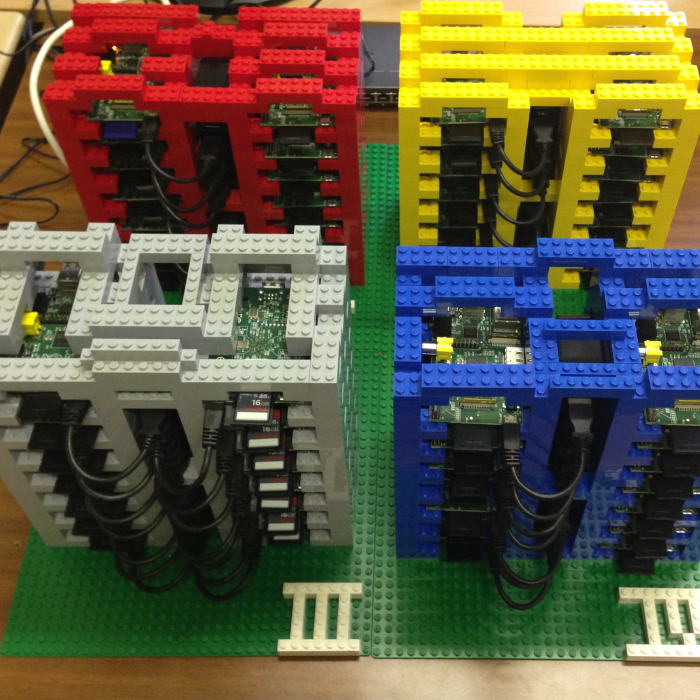
\includegraphics[width=0.5\textwidth]{picloud_towers}
	\caption{Photograph of the lego-built Raspberry Pi towers}
	\label{fig:pitowers}
\end{figure}

\section{University of Southampton Raspberry Pi Supercomputer}
\label{intro:pisupercomp}

It should be noted that University of Southampton also created a cluster of Raspberry Pi devices and before the University of Glasgow did according to the PiCloud blog \citep{picloudblog}, however theirs was designed to create a single, miniature super-computer.
This is sufficiently different in design and purpose from PiCloud as to disregard it for the purposes of this study.
